\documentclass{article}

% if you need to pass options to natbib, use, e.g.:
%     \PassOptionsToPackage{numbers, compress}{natbib}
% before loading neurips_2021

% ready for submission
\usepackage[final]{neurips_2021}

% to compile a preprint version, e.g., for submission to arXiv, add add the
% [preprint] option:
%     \usepackage[preprint]{neurips_2021}

% to compile a camera-ready version, add the [final] option, e.g.:
%     \usepackage[final]{neurips_2021}

% to avoid loading the natbib package, add option nonatbib:
%    \usepackage[nonatbib]{neurips_2021}

\usepackage[utf8]{inputenc} % allow utf-8 input
\usepackage[T1]{fontenc}    % use 8-bit T1 fonts
\usepackage{hyperref}       % hyperlinks
\usepackage{url}            % simple URL typesetting
\usepackage{booktabs}       % professional-quality tables
\usepackage{amsfonts}       % blackboard math symbols
\usepackage{nicefrac}       % compact symbols for 1/2, etc.
\usepackage{microtype}      % microtypography
\usepackage{xcolor}         % colors
\usepackage{amsmath}
\usepackage{verbatim}
\usepackage[mathscr]{euscript}
\usepackage{graphicx}
\title{Machine Learning, 2024 Spring\\Assignment 3}
% The \author macro works with any number of authors. There are two commands
% used to separate the names and addresses of multiple authors: \And and \AND.
%
% Using \And between authors leaves it to LaTeX to determine where to break the
% lines. Using \AND forces a line break at that point. So, if LaTeX puts 3 of 4
% authors names on the first line, and the last on the second line, try using
% \AND instead of \And before the third author name.



\begin{document}

\maketitle

\begin{abstract}

\end{abstract}

\textcolor{blue}{Problem 1}
For logistic regression, show that

\begin{equation}
    \nabla E_{\text {in }}(\mathbf{w})  =-\frac{1}{N} \sum_{n=1}^{N} \frac{y_{n} \mathbf{x}_{n}}{1+e^{y_{n} \mathbf{w}^{\mathrm{T}} \mathbf{x}_{n}}}  
 =\frac{1}{N} \sum_{n=1}^{N}-y_{n} \mathbf{x}_{n} \theta\left(-y_{n} \mathbf{w}^{\mathrm{T}} \mathbf{x}_{n}\right)
\end{equation}
Argue that a 'misclassified' example contributes more to the gradient than a correctly classified one.
\textcolor{blue}{Solution}


\newpage


\textcolor{blue}{Problem 2}
For linear regression, the out-of-sample error is 
\begin{equation}
    E_{\text{out}}(h)=\mathbb{E}[{(h(x)-y)}^2].
\end{equation}
Show that among all hypotheses, the one that minimizes $E_{\text{out}}$ is given by
\begin{equation}
    h^*(x)=\mathbb{E}[y|x].
\end{equation}
The function $h^*$ can be treated as a deterministic target function, in which case we can write $y=h^*(x)+\epsilon(x)$ where $\epsilon(x)$ is an (input dependent) noise variable. Show that $\epsilon(x)$ has expected value zero.
\newline
\textcolor{blue}{Solution}

\newpage

\textcolor{blue}{Problem 3}
According to the iterative format provided as follow:
\begin{itemize}
    \item Use the SUV dataset to implement (using Python or MATLAB) the Gradient Descent method to find the optimal model for logistic regression.
    \item What is your test error? What are the sizes of the training set and test set, respectively?
    \item What is your learning rate? How was it chosen? How many steps were iterated in total?
    \item Present the results of the last 10 steps produced by your algorithm, including the loss, learning rate, the L2 norm of the gradient, and the number of function evaluations and gradient evaluations.
\end{itemize}
\begin{figure}[htbp]
\centerline{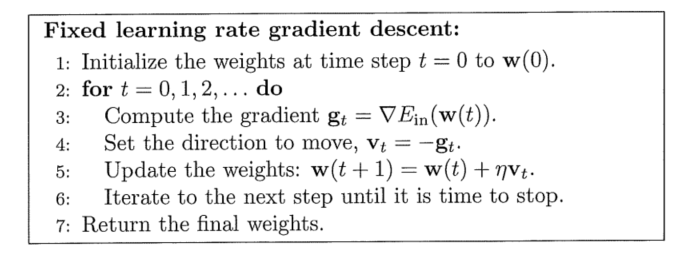
\includegraphics[width=0.8\textwidth]{alg.png}}

\href
  {https://www.cs.toronto.edu/~mhsadi/code-repository/MachineLearningNotebooks/3-SUVDataset.html}
  {Dataset reference and description}
  \\
\href
{https://www.kaggle.com/datasets/iamaniket/suv-data?resource=download}
  {Dataset and download}

\end{figure}


\textcolor{blue}{Solution}






\end{document}